%!TEX root = ../../thesis.tex
\section{Continuous state space}
\label{chapter:limitations:continousstate}

\question{How to leverage from the discrete set of state constrain?}

As for now, our algortihm assume the world can be represented by a limited number of discrete states. In this section we extend our algorithm to a continuous world, however we still conider discrete action. In additon, we present anew interaction frame that combines the feedback and guidance instructions. We investigate how our algorithm scales to such problem and how different exploration strategies perform.

\subsection{Experimental System}

We consider a world which is known in the reinforcement learning literature as the \emph{puddle world}. The puddle world consist in a continuous-state MDP in which an agent must reach a goal region while avoiding a penalty region. We consider a 2 dimensional puddle world with each dimension ranging between 0 and 1. Agent actions are discrete and represent steps in either North, South, East, West direction. One step length is sampled from a normal distribution of mean 0.1 and standard deviation 0.01.

As in the experiment of chapter~\ref{chapter:lfui}, we consider speech as the modality for interacting with the robot and we reuse the dataset presented in chapter~\ref{chapter:lfui:speechdata}. The interaction between the agent and the teacher follows a turn taking social behavior, where the agent is performing an action and waits for a feedback or guidance signal to continue. We only consider a Gaussian classifier.

\paragraph{Task Representation} 

To define the set of possible tasks we project a 5x5 regular grid on top of the continuous world. One task is represented by a +1 reward in one of the 25 projected squares and a -100 reward in three consecutive (vertically or horizontally) squares. +1 and -100 area can not overlap (see figure~\ref{UncertaintyMap}(E) for an example). The set of possible task is defined as all possible combination of such reward function, for a total of 660 hypothesis. 

Our algorithm only need to have access to the optimal policies to be able to interpret a signal with respect to the feedback or guidance frame. We use the MDP framework to compute the corresponding policies. The world being continuous we use the tile coding function approximation \cite{sutton1998reinforcement}, with 10 overlapping 50x50 regular grids. 

A Q-Learning algorithm \cite{watkins1992q} is used to compute the Q-Values, with a discount rate of 0.99 and a learning rate of 0.01. The  optimal policies are then defined as greedy according to the Q-Values.

\paragraph{Mixed feedback and guidance frame}

In previous chapter we considered only the feedback or the guidance frame separately. Such limitation can be restrictive for the user, we will now consider the case where the teacher can use both feedback and guidance signal. We define as $F$ as the set of meanings associated to the feedback meanings (i.e. ``correct'' and ``incorrect''), and $G$ the set of meanings associated to the guidances meanins (i.e. ``action 1'', ``action 2'', ...). Extending our algorithm to cases where possible meanings include both feedback and guidance (i.e. $l^f \in \{F \cup G\}$) requires a probabilistic model of how the teacher distribute feedback and guidance signals. This model must hold the following property $\sum_{l \in \{F \cup G\}} p(l^f = l|s,a,\xi)~=~1$. We define a variable $\phi$ that represents the probability of the user providing a feedback signal at each step, i.e. $p(l^f \in F) = \phi$, which implies $p(l^f \in G) = 1 - \phi$. 

Under this new definition we can change our frame definition to:

\begin{eqnarray}
    p(l^f = l|s,a,\xi) = 
        \begin{cases} 
            \phi~p(l^f = l|s,a,\xi) &\mbox{for } l \in F \\
            (1- \phi)~p(l^f = l|s,\xi) & \mbox{for } l \in G
        \end{cases}
        \label{eq:mixedfeedbackguidance}
\end{eqnarray}
where Equation~\ref{eq:feedbackframe} holds for the feedback component (for $l \in F$) and Equation~\ref{eq:guidanceframe} holds for the guidance component (for $l \in G$). 

We assume the mixing parameter $\phi$ is known in advance. We set $\phi$ to 0.5 meaning the user is providing feedback half of the time and guidance the other half of the time. 

\paragraph{Exploration strategies}

We will investigate four different agent behaviors: \begin{inparaenum}[a)] \item random, \item $\epsilon$-greedy, \item myopic uncertainty based exploration, which aims at selecting the action that is the most uncertain in the current state, and \item full uncertainty based exploration which requires an uncertainty map to decide what to explore next. \end{inparaenum} 

As we are in a continuous domain we can not compute the full uncertainty for each state as presented in chapter~\ref{chapter:planning}, we therefore approximate this process. Extensions of the general problem already exist for the continuous state problem \cite{nouri2010dimension,Hester13aamas} and we will rely on a sampling based method. One hundred random states are generated and evaluated in terms of uncertainty. Each sampled state is associated to a reward value proportional to its uncertainty which is propagated to neighborhood states by using a fixed Gaussian kernel. We use as amplitude the uncertainty value and a diagonal covariance matrix of value 0.01 for each component. The resulting approximated uncertainty map is then used as a reward function in a our MDP. By solving this problem, using for instance Q-Learning, the agent plans its actions to visit the most uncertain regions. We then decided to use an $\epsilon$-greedy policy on the Q-values. In the following experiment, the agent will use an exploration ratio $\epsilon$ equal to $0.1$.

\subsection{Results}

We present results from 75 runs of our experiment, where for each run we randomly choose a task to teach from the set of hypothesis as well as the initial state of the agent. The simulated teacher was making 10 percent of teaching mistake, i.e. sending an erroneuous signal 10 percent of the time. For each experiment, we compute the likelihoods every 15 steps and performs a total of 35 updates, for a total of 525 iterations. Figure~\ref{fig:continuousstateRmax} shows the average evolution of the taught task hypothesis likelihood.

\begin{figure}[!ht]
  \centering
  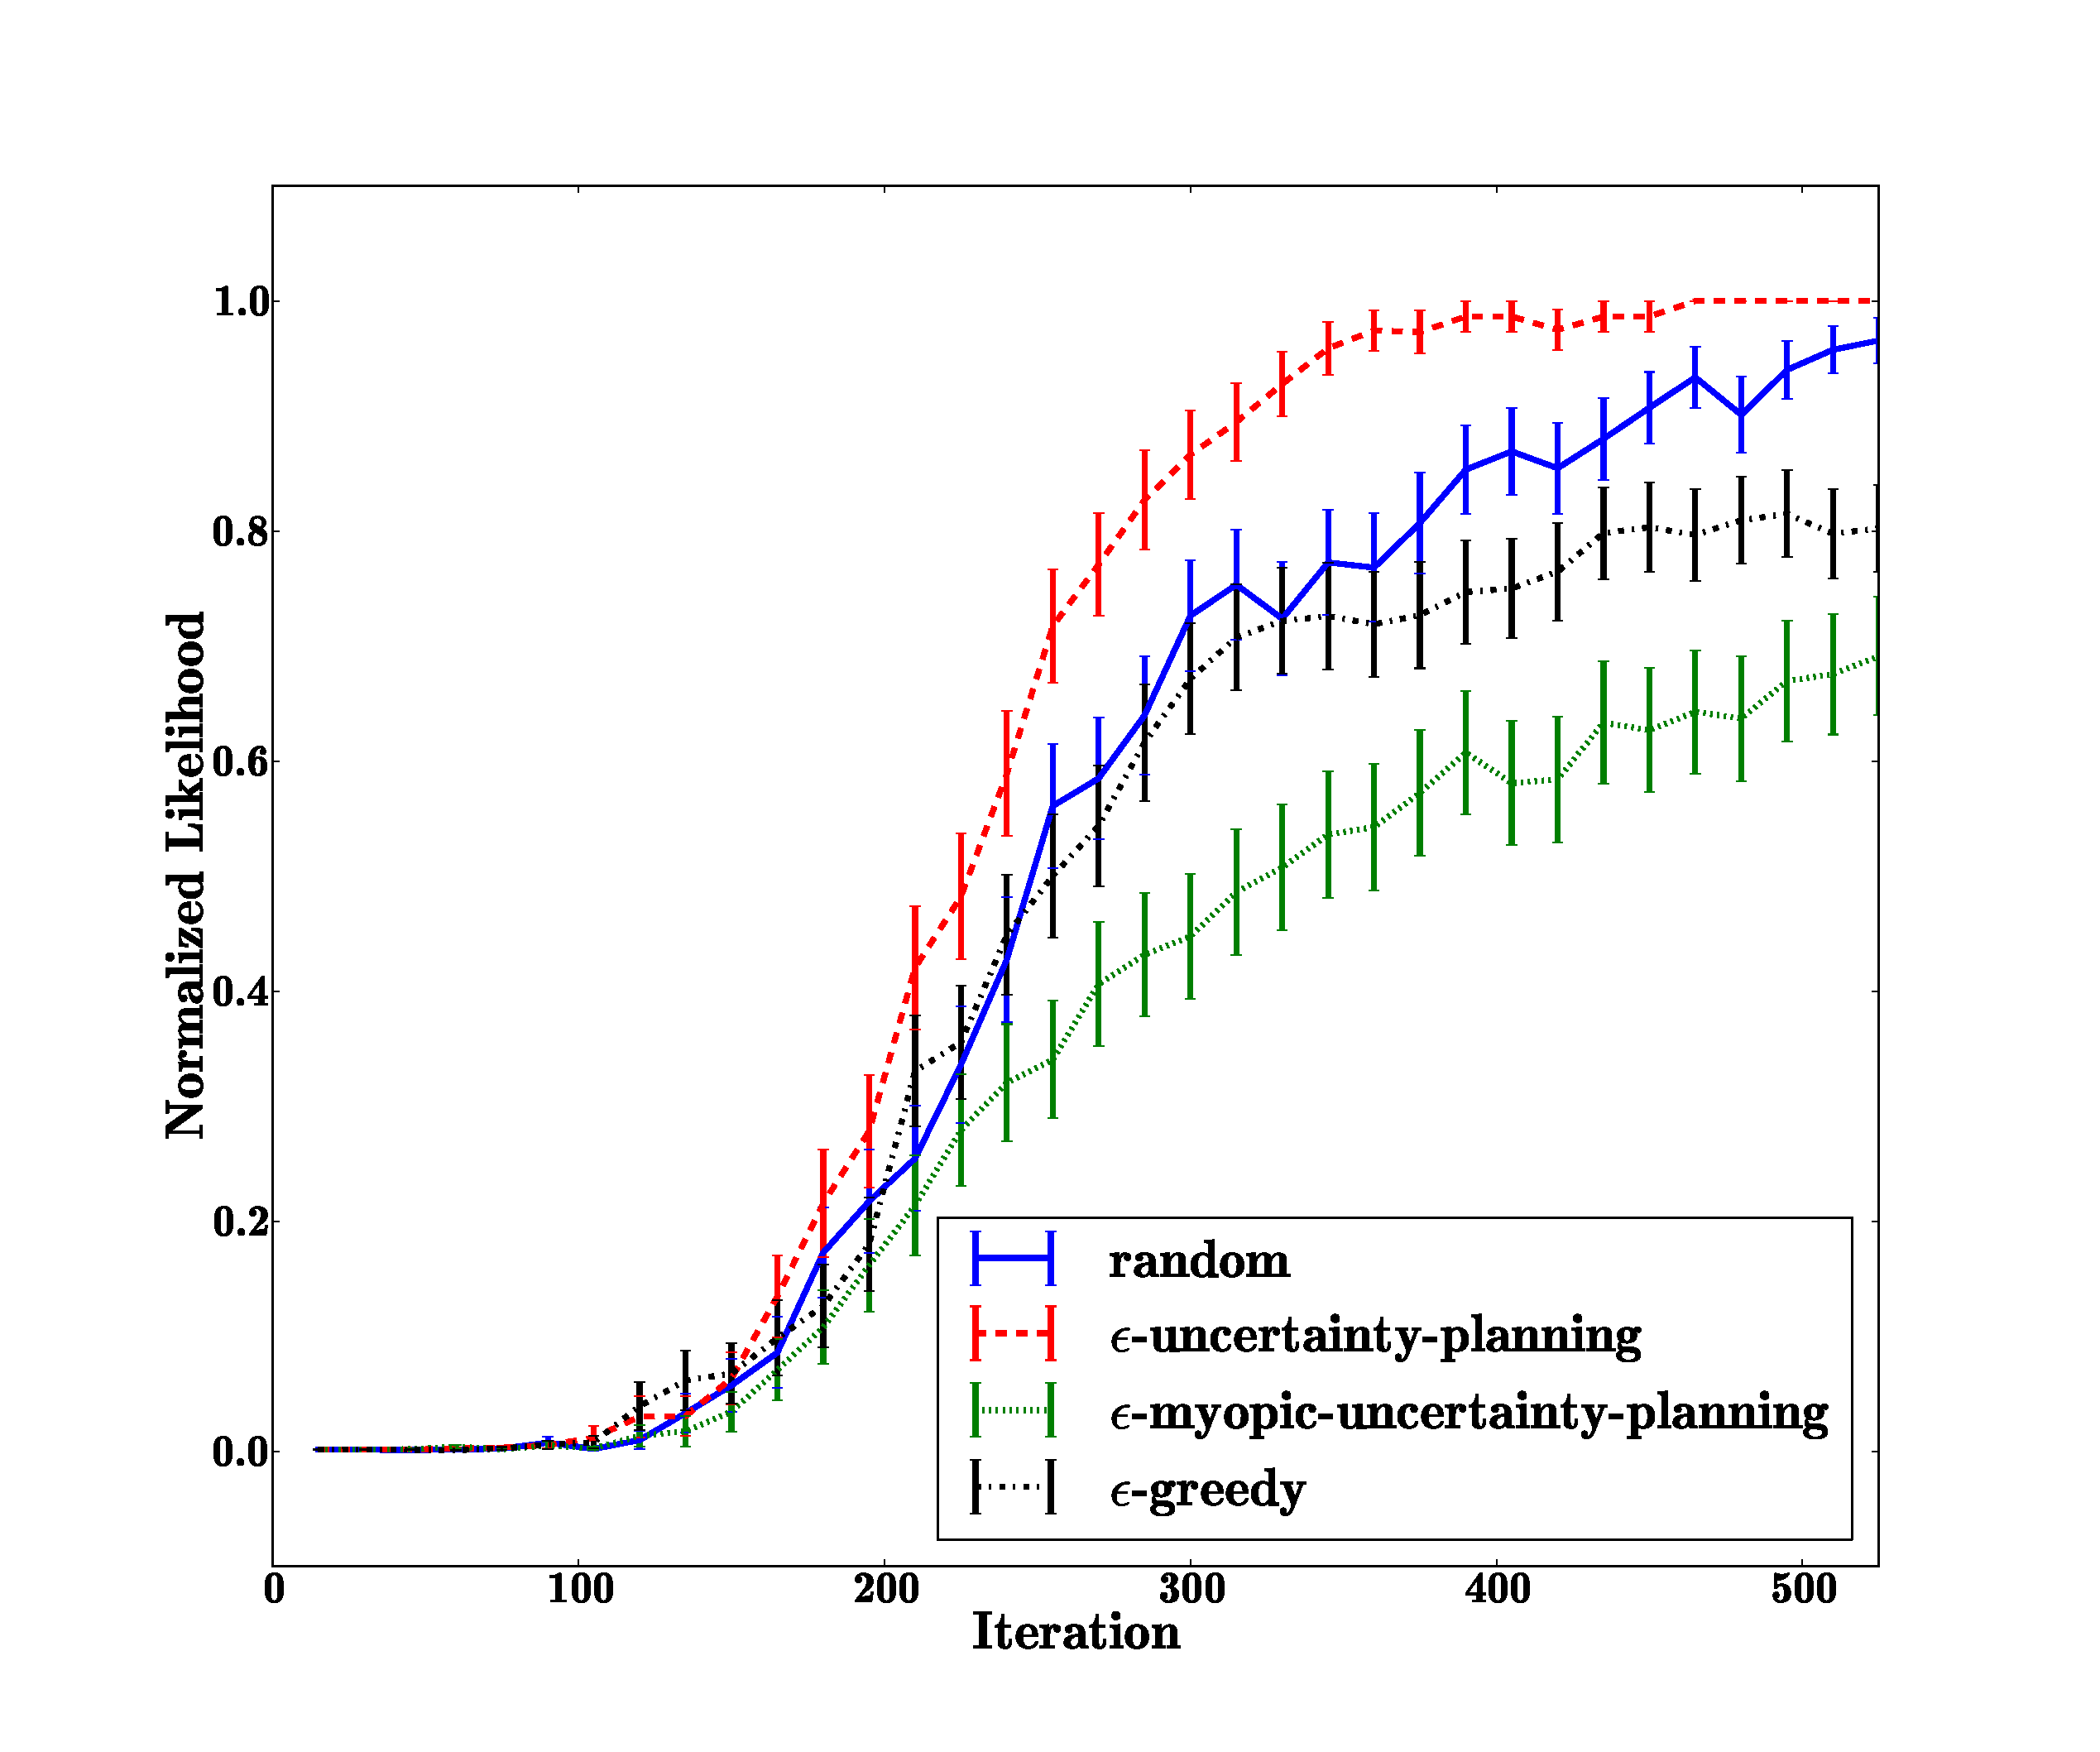
\includegraphics[width=\plotsize\columnwidth]{\imgpath/continuous_state/continuous}
  \caption{Taught hypothesis normalized likelihood evolution (mean + standard error) thought iteration using a Gaussian classifer. Comparaison of different exploration strategies. Uncertainty based exploration method, which plan on the long term, performs significantly better on average.}
  \label{fig:continuousstateRmax}
\end{figure}

Those results show that our algorithm can learn a task in a continuous world from unlabeled and noisy instructions whose possible meanings are both feedback and guidance and 10 percent of the instructions were teaching mistakes. The uncertainty based planning strategy outperforms random action selection. Interestingly, myopic uncertainty based strategy, which is also based on our uncertainty measure, is not efficient. This result illustrates that, when considering the agent as not being able to teleport, a long term planning approcah is more suited to explore efficiently the state space than a short term vision by selecting the next action with higher immediate reward, i.e. the state-action pair with higher uncertainty given the state of the agent. 

% Finally $\epsilon$-greedy performs less efficiently than in the first setup. This is due to the properties of our new set of hypothesis where many hypothesis shared an identical positive reward area but have different puddle zone.

Figure~\ref{fig:continuousstateUncertaintyMap} shows the evolution of the estimated uncertainty map for one run of the experiment. For each uncertainty map, the agent plans its actions to reach a maximal uncertainty region. The maximum uncertainty value decreases as the agent is correctly estimating the task.

\begin{figure}[!ht]
  \centering
      \begin{subfigure}[b]{0.35\columnwidth}
          \centering
          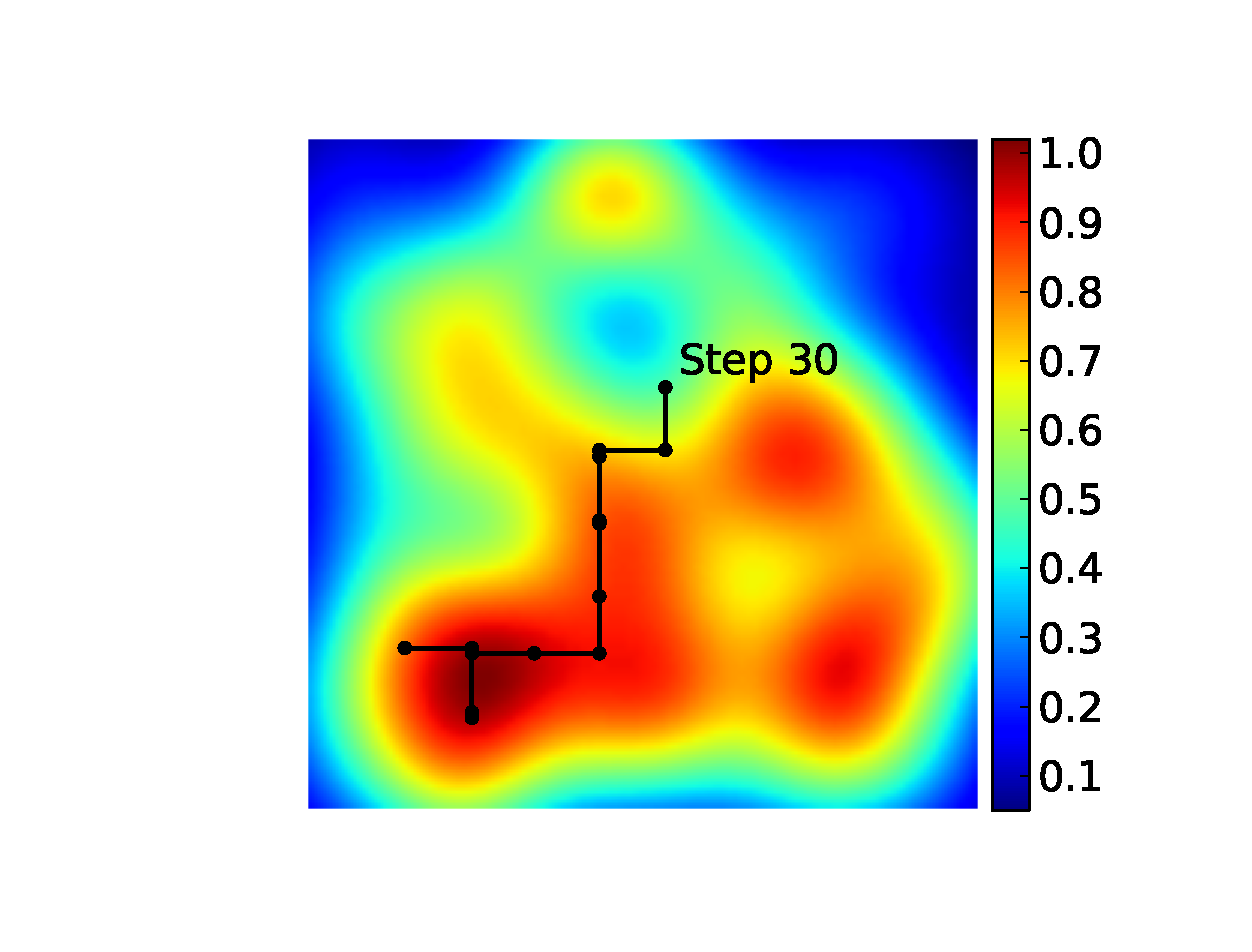
\includegraphics[trim=5cm 1.5cm 1.5cm 1.5cm, clip=true, width=\columnwidth]{\imgpath/continuous_state/30}
          \caption{After 30 iterations.}
          \label{fig:30}
      \end{subfigure}
      \begin{subfigure}[b]{0.35\columnwidth}
          \centering
          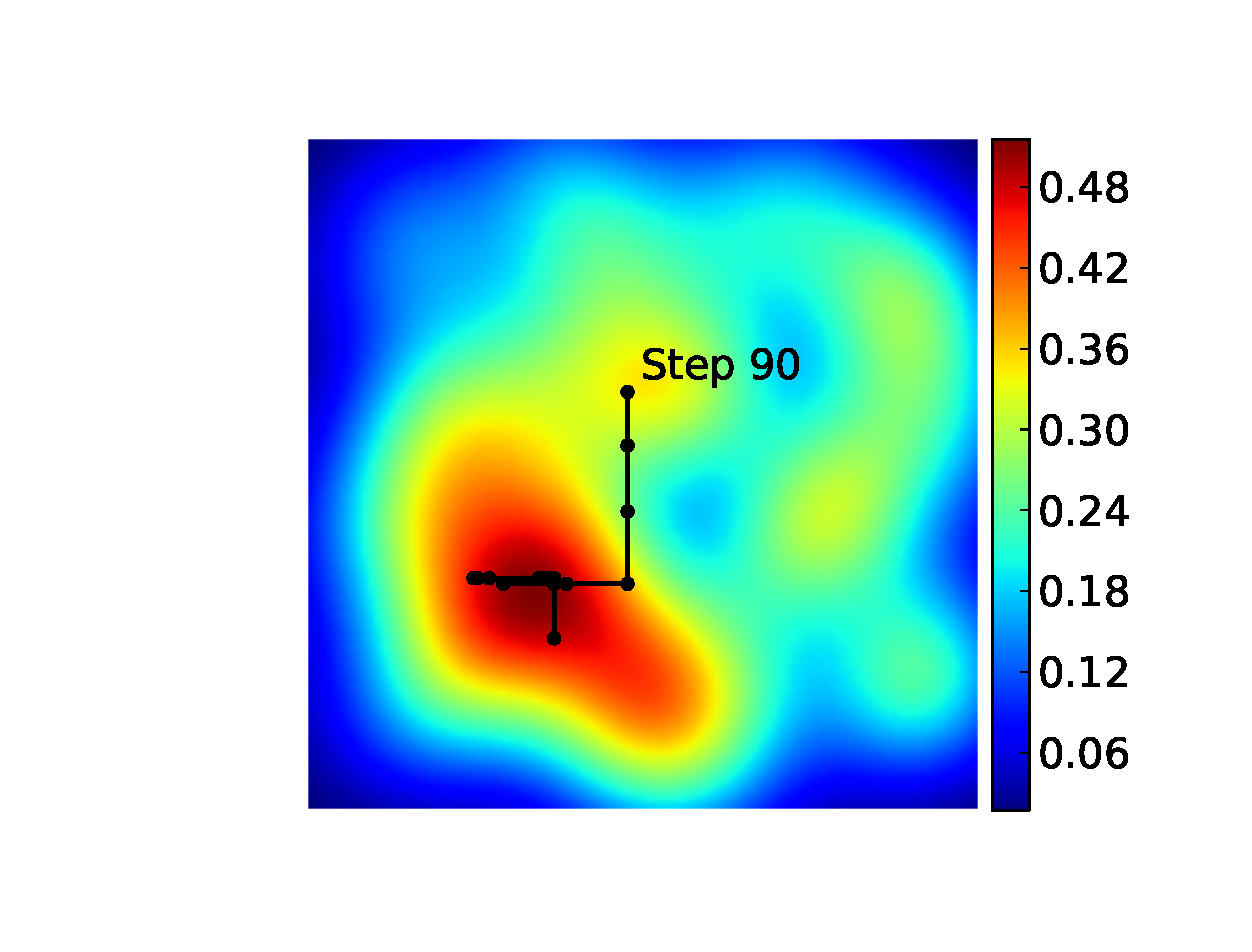
\includegraphics[trim=5cm 1.5cm 1.5cm 1.5cm, clip=true, width=\columnwidth]{\imgpath/continuous_state/90}
          \caption{After 90 iterations.}
          \label{fig:90}
      \end{subfigure}\\
      \begin{subfigure}[b]{0.35\columnwidth}
          \centering
          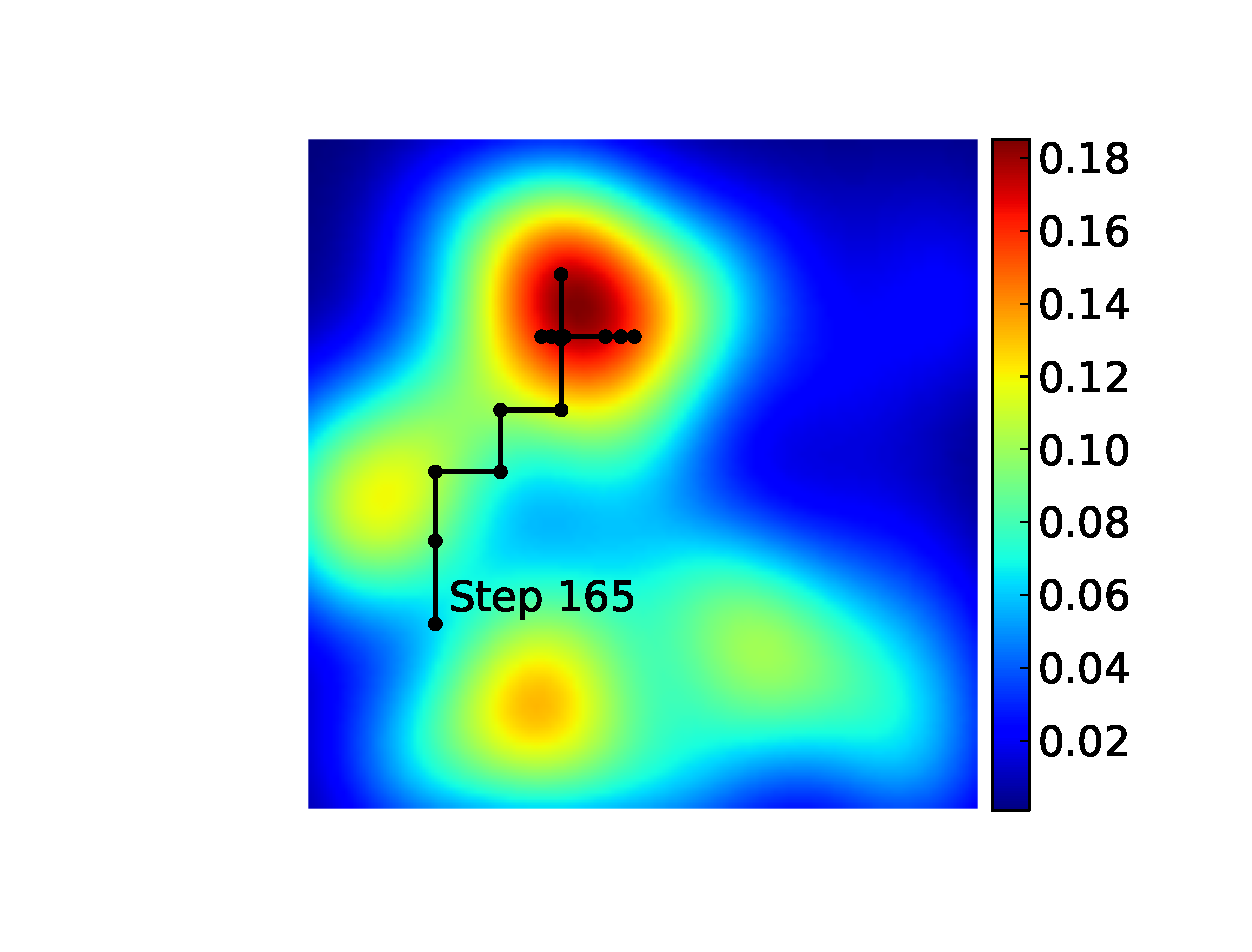
\includegraphics[trim=5cm 1.5cm 1.5cm 1.5cm, clip=true, width=\columnwidth]{\imgpath/continuous_state/160}
          \caption{After 165 iterations.}
          \label{fig:165}
      \end{subfigure}
      \begin{subfigure}[b]{0.35\columnwidth}
          \centering
          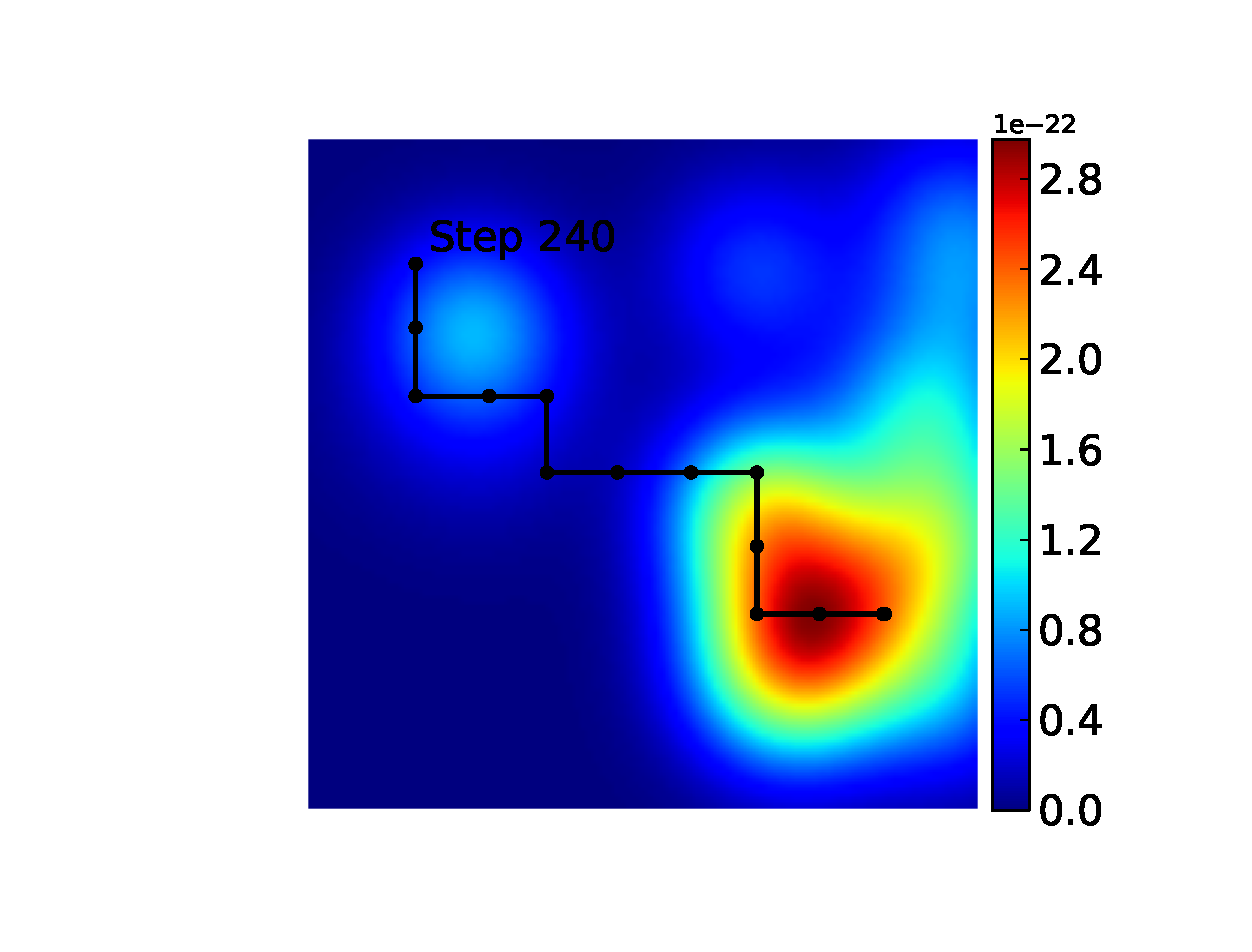
\includegraphics[trim=5cm 1.5cm 1.5cm 1.5cm, clip=true, width=\columnwidth]{\imgpath/continuous_state/240}
          \caption{After 240 iterations.}
          \label{fig:240}
      \end{subfigure}\\
      \begin{subfigure}[b]{0.25\columnwidth}
          \centering
          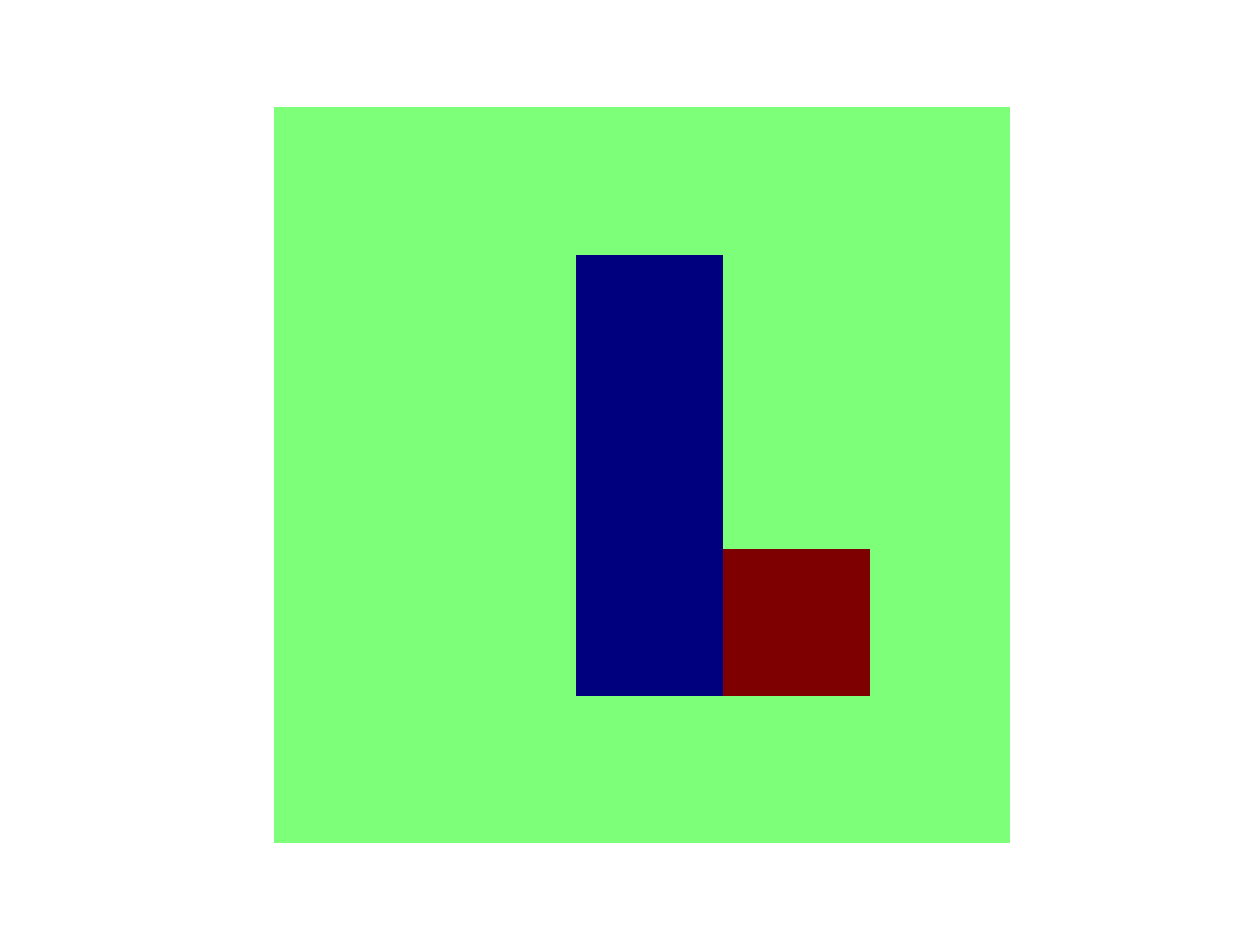
\includegraphics[trim=4cm 1cm 3.5cm 1cm, clip=true, width=\columnwidth]{\imgpath/continuous_state/puddle}     
          \caption{Puddle world used by the teacher.}
          \label{fig:puddle}
      \end{subfigure}
      \begin{subfigure}[t]{0.45\columnwidth}
          \centering
          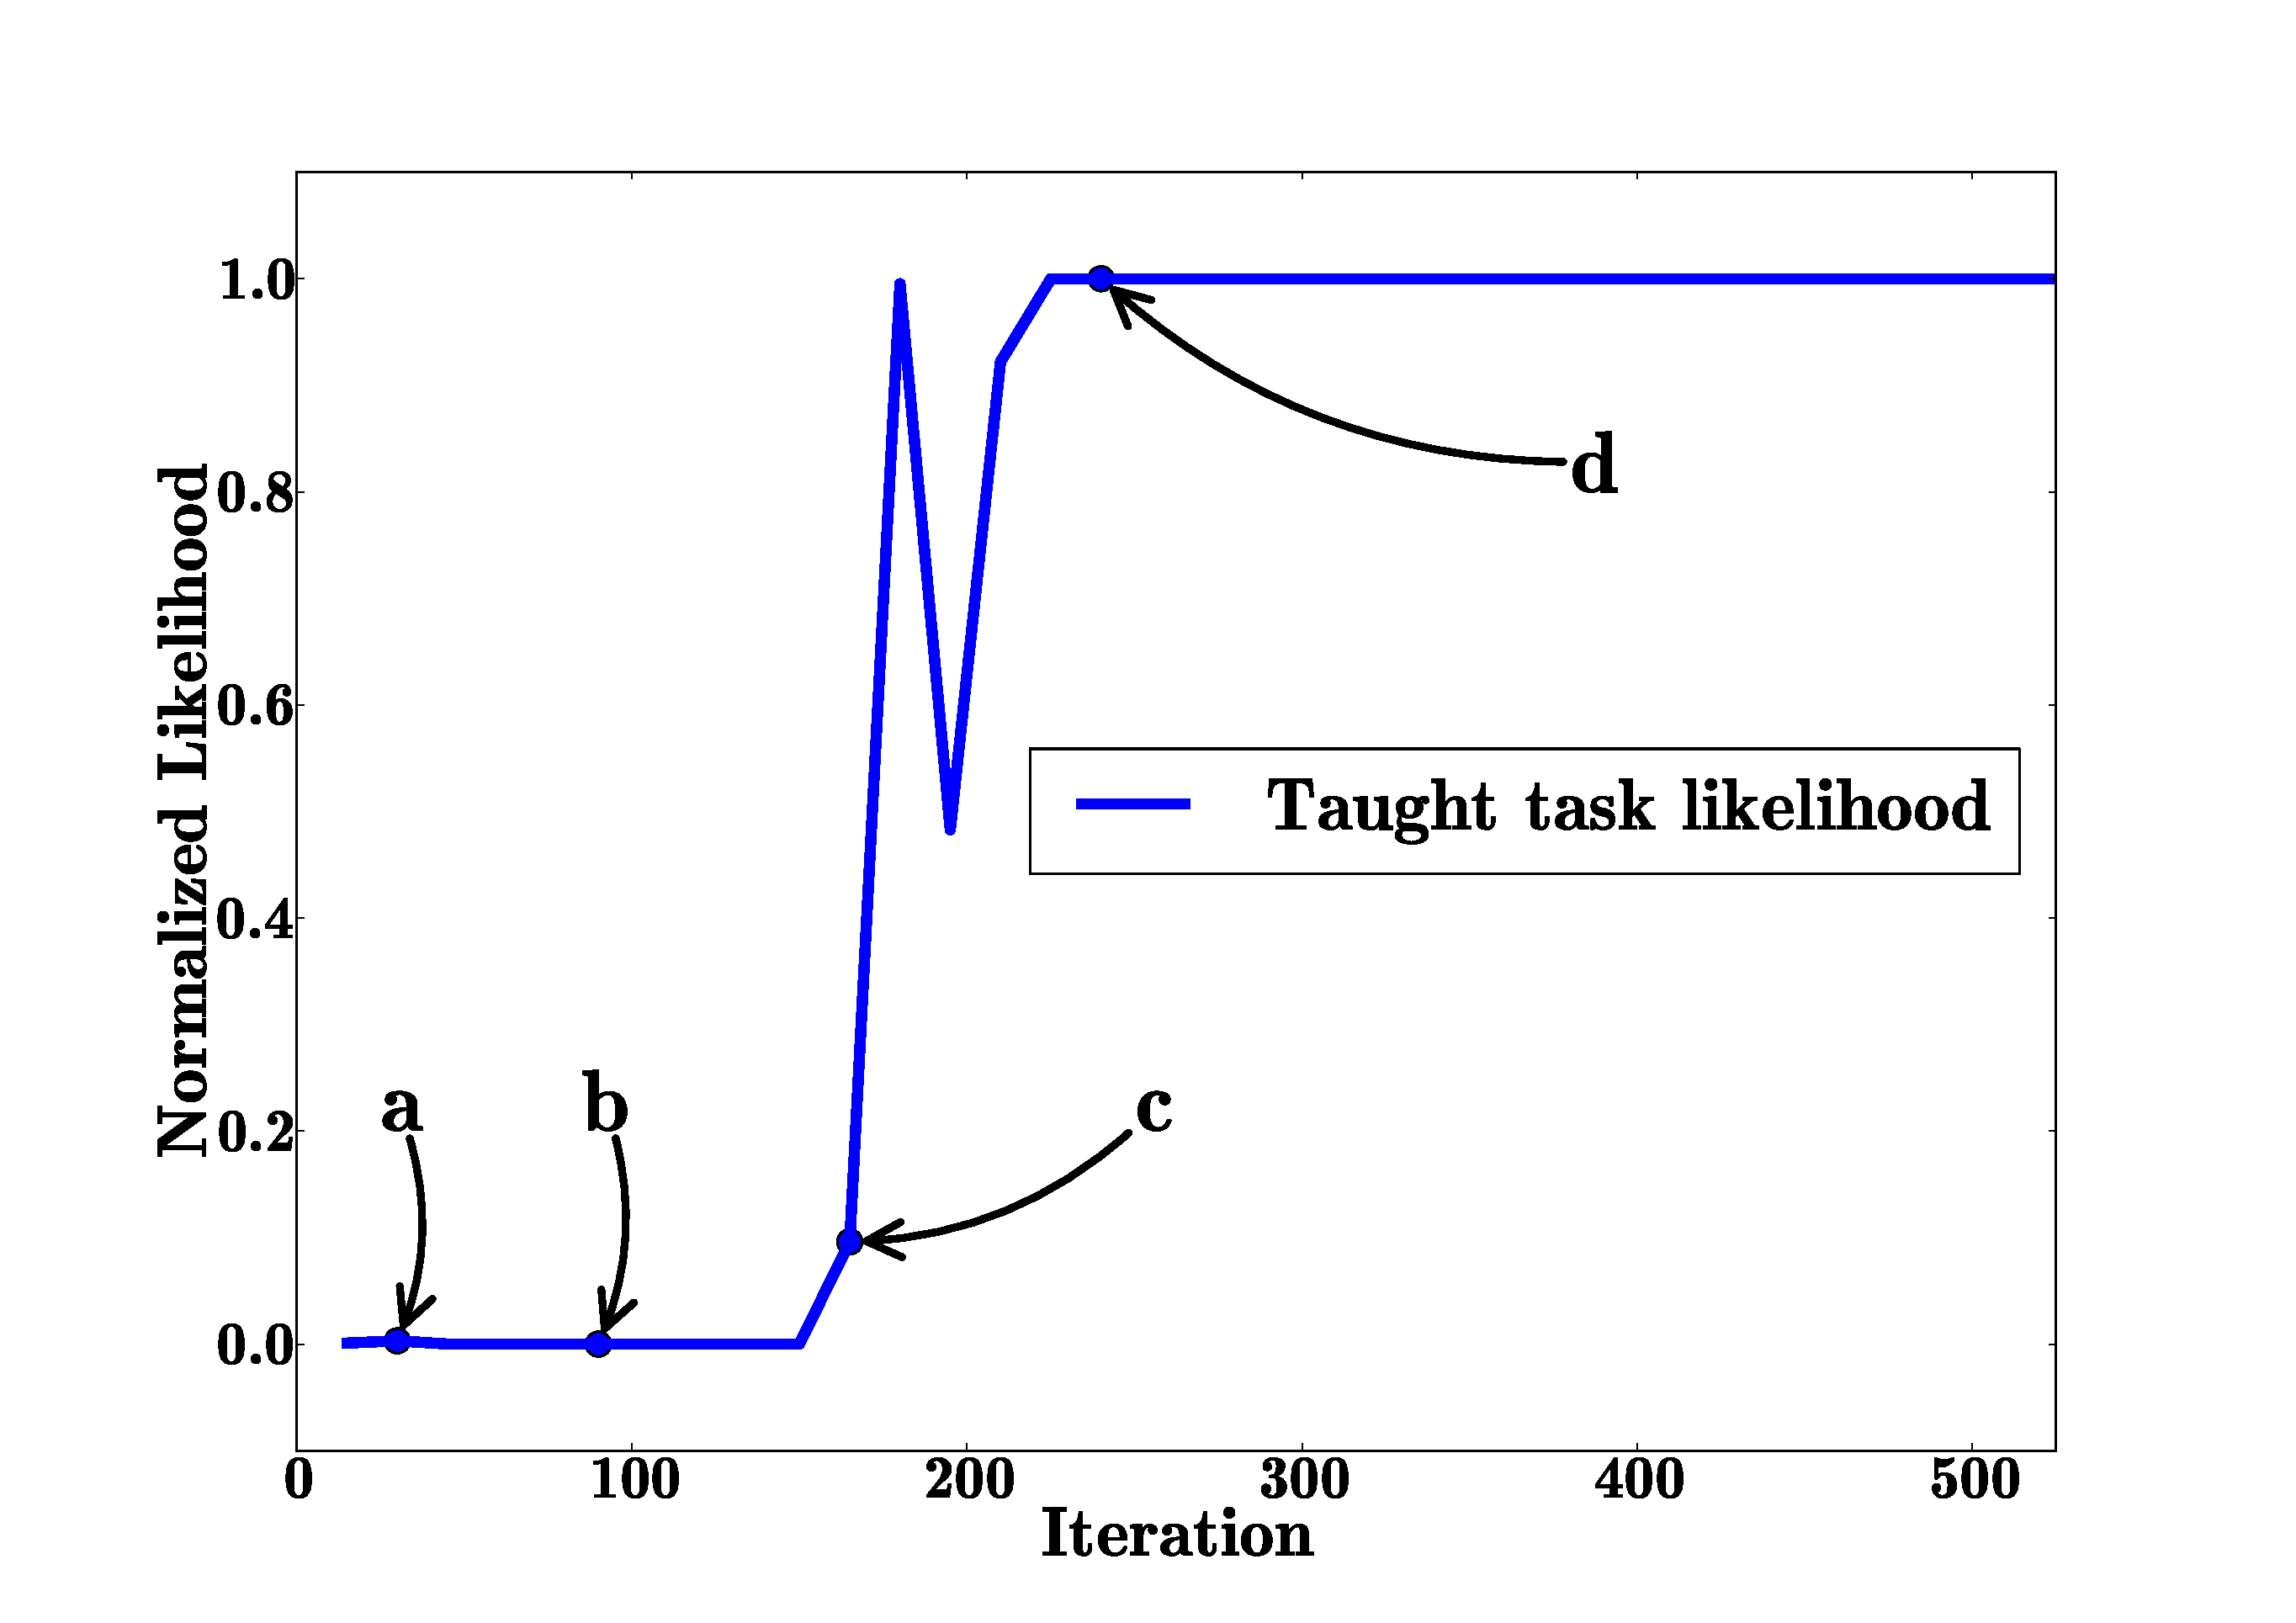
\includegraphics[trim=2cm 1cm 3cm 2cm, clip=true, width=\columnwidth]{\imgpath/continuous_state/evo}
          \caption{Taught hypothesis normalized likelihood evolution.}
          \label{fig:evo}
      \end{subfigure}
        
  \caption{Log Uncertainty maps after a) 30, b) 90, c) 165 and d) 240 iterations. e) shows the puddle world choosen by the teacher and f) shows the learning progress and the frame associated to each of the uncertainty map. In order to display the differences between log values, we bounded the colormap between -5 and 0, which correspond to uncertainty values between 0.0067 and 1. Some log values, especially for d), are lower than -5 and are displayed in the same color as -5. Best shown in color.}
  \label{fig:continuousstateUncertaintyMap}
\end{figure}